
\section*{第一章\ 論文格式與目錄設定}
\addcontentsline{toc}{section}{第一章\ 論文格式與目錄設定}

\subsection*{1.1\ 標號}
\addcontentsline{toc}{subsection}{1.1\ 標號}
插入圖片之後，在要加上編號的地方，點選「參考資料」/「標號」/「插入標號」。第一次新增標號時，要點選「新增標籤」，輸入「圖」或「表」，之後只要在標籤裡選擇「圖」或「表」即可，如果有設定好大綱編號，可以在編號方式中將「包含章節編號」打勾，在這個範本第幾章是使用標題1，所以章節起始樣式選標題1，按確定，插入標號後，按一下tab (不要使用空白，以免影響到圖目錄的對齊)，接著在後面打上想要的說明即可。
\textbf{}\\
\begin{figure}[h]
    \centering
    
\includegraphics[width=.8\textwidth]{figure1.png} %圖片文件的路徑
    \addcontentsline{lof}{figure}{Figure1.1\ 插入標號的路徑} 
    \caption*{Figure1.1\ 插入標號的路徑}
    \label{img} 
\end{figure}
\begin{figure}[h]
    \centering %置中
    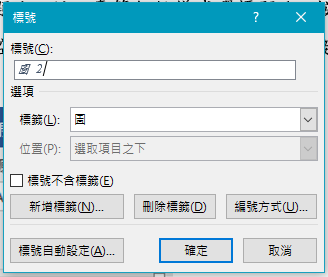
\includegraphics[width=.8\textwidth]{figure2.png}
    \addcontentsline{lof}{figure}{Figure1.2\ 標號設定} 
    \caption*{Figure1.2\ 標號設定} 
    \end{figure}
\clearpage

\subsection*{1.2\ 標題及內文格式}
\addcontentsline{toc}{subsection}{1.2\ 標題及內文格式}
中文字型需為標楷體、西文字型則為 Times New Roman。
\textbf{}\\
\begin{table}[h]
    \caption*{Table1.1\ 學院與所屬字體顏色}
    \addcontentsline{lot}{table}{Table1.1\ 學院與所屬字體顏色}
    \definecolor{light-silver-blue}{RGB}{176, 196, 222} %latex預設顏色無淺銀灰藍色，調整並定義淺銀灰藍色字體
    \begin{tabular}{|c|c|}
    \hline
    \rowcolor[HTML]{D9D9D9} 
    \begin{tabular}[c]{@{}c@{}}各院名稱\\ College of Name\end{tabular}        
    & \begin{tabular}[c]{@{}c@{}}精裝論文顏色\\ Color(tooled in gold font)\end{tabular} \\ \hline
    \begin{tabular}[c]{@{}c@{}}理學院\\ College of Science\end{tabular}      
    & {\color[HTML]{000000} \begin{tabular}[c]{@{}c@{}}{\color{blue}藍色} (燙金字體)\\ {\color{cyan}Blue}(tooled in gold font)\end{tabular}}\\ \hline
    \begin{tabular}[c]{@{}c@{}}工學院\\ College of Engineering\end{tabular}  
    & \begin{tabular}[c]{@{}c@{}}黑色(燙金字體)\\ Black(tooled in gold font)\end{tabular}\\ \hline
    \begin{tabular}[c]{@{}c@{}}商學院\\ College of Business\end{tabular}     
    & \begin{tabular}[c]{@{}c@{}}{\color{green}綠色}(燙金字體)\\ {\color{green}Green} (tooled in gold font)\end{tabular}   \\ \hline
    \begin{tabular}[c]{@{}c@{}}設計學院\\ College of Design\end{tabular}      
    & \begin{tabular}[c]{@{}c@{}}{\color{brown}咖啡色}(燙金字體)\\ {\color{brown}Brown}(tooled in gold font)\end{tabular}\\ \hline
    \begin{tabular}[c]{@{}c@{}}人育學院\\ College of Humanities and Education\end{tabular} 
    & \begin{tabular}[c]{@{}c@{}}{\color{red}紅色}(燙金字體)\\ {\color{red}Red}(tooled in gold font)\end{tabular}\\ \hline
    \begin{tabular}[c]{@{}c@{}}電資學院\\ College of Electrical Engineering \\ and Computer Science\end{tabular} 
    & \begin{tabular}[c]{@{}c@{}}{\color{light-silver-blue}淺銀灰藍色}(燙金字體)\\ {\color{light-silver-blue}Silver gray blue}(tooled in gold font)\end{tabular}\\ \hline
    \begin{tabular}[c]{@{}c@{}}法學院\\ School of Law\end{tabular}           
    & \begin{tabular}[c]{@{}c@{}}{\color{red}暗紅色}(燙金字體)\\ {\color{red}dark red}(tooled in gold font)\end{tabular}\\ \hline
    \end{tabular}
\end{table}
\begin{table}[h] %[h]為表格排版
\caption*{Table1.2\ 格式說明}
\addcontentsline{lot}{table}{Table1.2\ 格式說明}
\begin{tabular}{|l|l|l|}
\hline
類別  & 字體大小 & 編號方式 \\ \hline
內文  & 12   & 無    \\ \hline
標題一 & 18   & 第*章  \\ \hline
標題二 & 16   & 第*節  \\ \hline
標題三 & 14   & *、   \\ \hline
圖表  & 9    & 標號   \\ \hline
\end{tabular}
\end{table}
\clearpage

\subsection*{1.3\ 新增圖、表目錄方式}
\addcontentsline{toc}{subsection}{1.3\ 新增圖、表目錄方式}
在「參考資料」之「標號」中，點選插入「圖表目錄」，然後選擇「標題標籤」即可。
\textbf{}\\
\begin{figure}[h]
 \centering %置中
 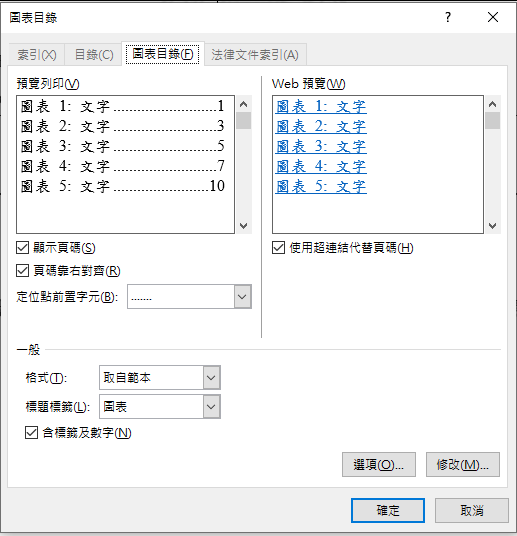
\includegraphics[width=.8\textwidth]{figure3.png}
\caption*{Figure1.3\ 插入圖表目錄}
\addcontentsline{lof}{figure}{Figure1.3\ 插入圖表目錄}
\end{figure}
\clearpage